% =====================================================================
%  RESULTADOS
%  Cifras de RESULTADOS_OE4_SIMULACION.md y de la evidencia de hardware
%  S24_peldano2 / S24_nav2_navegacion / S25_pisos34_campo.
%
%  Las tres cosas que hay que escribir con cuidado van en §4.4:
%   - R14: la continuidad es un invariante, no un resultado experimental
%   - El intervalo de Wilson: «supera el 70 %», no «es del 86,7 %»
%   - R15: la campaña corrió con un mapa que leía libre lo desconocido
% =====================================================================
\chapter{Resultados}

\begin{notaavance}[la toma de datos cierra el 16 de octubre de 2026]
Las cifras de este capítulo son las disponibles al \textbf{5 de octubre de
2026}. Las dos mitades están en situaciones distintas y conviene no leerlas
igual:

\begin{itemize}[leftmargin=*,nosep]
  \item El §4.1, \textbf{simulación}, está \textbf{cerrado}. La campaña de
    treinta misiones corrió el 5 de septiembre, el analizador la dictaminó
    válida y sus números no van a cambiar.
  \item El §4.2, \textbf{hardware}, \textbf{va por mitades}. La odometría
    (compuerta G-2) cerró el 5 de octubre y se reporta. La precisión de llegada
    (G-3) no se alcanzó en el corte C-1 y sigue abierta, así que ese apartado
    queda sin redactar hasta el corte del \textbf{viernes 16 de octubre},
    después del cual el acta de directores no admite más datos.
\end{itemize}

El §4.3 trata de las limitaciones de la campaña de simulación, así que cierra
con ella.
\end{notaavance}

Los resultados llegan de dos campañas distintas. La primera, en simulación, con
treinta misiones sorteadas. La segunda, sobre los vehículos reales en los
pasillos del edificio. Se reportan por separado porque miden cosas distintas: la
de simulación mide el sistema completo con relevo, la de hardware mide hasta
dónde llega la plataforma física.

% ---------------------------------------------------------------------
\section{Evaluación en simulación}

La campaña corrió treinta misiones sorteadas, quince de control dentro de un
mismo nivel y quince entre niveles. El analizador dictaminó \textbf{campaña
válida}, con \textbf{cero descartes} contra un techo admitido del 20~\%.

\subsection{Tasa de éxito (RF-23)}

Una misión es exitosa si cumple dos cosas. Que la pose final quede a 0,25~m o
menos del destino, medida contra la odometría y no contra el resultado de Nav2.
Y que la misión llegue a completarse sin pasar por fallo.

\begin{table}[H]
  \centering\small
  \caption{Tasa de éxito de la campaña, con intervalo de confianza de Wilson.}
  \label{tab:exito}
  \begin{tabular}{@{}lcccc@{}}
    \toprule
    & \textbf{n} & \textbf{éxitos} & \textbf{tasa} & \textbf{IC 95 \% (Wilson)} \\ \midrule
    Campaña completa & 30 & 26 & \textbf{86,7 \%} & \textbf{70,3 -- 94,7 \%} \\
    Condición A — control & 15 & 12 & 80,0 \% & 54,8 -- 93,0 \% \\
    Condición B — inter-nivel & 15 & 14 & 93,3 \% & 70,2 -- 98,8 \% \\ \bottomrule
  \end{tabular}
\end{table}

\textbf{La afirmación defendible es que la tasa de éxito supera el 70~\%}, no que
sea del 86,7~\%. Con treinta misiones el intervalo mide 24 puntos porcentuales de
ancho, y ese límite es de diseño: no se arregla trabajando más, se arreglaría con
más muestra. El 86,7~\% es el estimador puntual y se reporta siempre junto a su
intervalo.

Los dos intervalos de las condiciones se solapan, así que \textbf{la comparación
entre ellas no sostiene ninguna conclusión}. Conviene decirlo porque el estimador
puntual apunta en contra de la intuición: la condición con relevo salió mejor que
la de control.

\subsection{Los cuatro fallos son un solo modo}

Las cuatro misiones fallidas quedaron a 0,295, 0,284, 0,311 y 0,347~m del
destino, contra una tolerancia de 0,25~m. Las cuatro se quedaron \emph{cortas},
ninguna se pasó ni terminó en otro sitio.

Eso no es un fallo de coordinación: es el límite de precisión de la aproximación
final. El error de llegada del conjunto tiene mediana \textbf{0,106~m} y recorrido
de 0,019 a 0,347~m.

\subsection{Tiempo de respuesta (RF-21) y de asignación (RF-22)}

El tiempo de respuesta se reporta por escalones y no con media y desviación, por
una razón de instrumento:

\begin{table}[H]
  \centering\small
  \caption{Tiempo de respuesta, en escalones del reloj de simulación.}
  \label{tab:respuesta}
  \begin{tabular}{@{}lcccc@{}}
    \toprule
    \textbf{t respuesta} & 0,1 s & 0,2 s & 0,3 s & 0,4 s \\ \midrule
    misiones & 10 & 15 & 4 & 1 \\ \bottomrule
  \end{tabular}
\end{table}

Los cuatro valores son múltiplos exactos de 100~ms, que es el tic del reloj de
simulación. \textbf{La resolución del instrumento vale entre el 25~\% y el 100~\%
de la magnitud medida.} Una mediana de 0,2~s significa «uno o dos tics», no
«doscientos milisegundos». Dar media y desviación sugeriría una precisión que el
reloj no entrega.

Lo que sí se sostiene es la cota, que además es lo que le importa a un usuario:
\textbf{el robot arranca en menos de medio segundo}.

El tiempo de asignación quedó por debajo de 100~ms en las treinta. Como esa cifra
cae tres órdenes de magnitud por debajo de un tic del reloj, se caracterizó
aparte en banco: mediana entre 154 y 175~\textmu s, máximo 306~\textmu s.

% ---------------------------------------------------------------------
\begin{figure}[H]
  \centering
  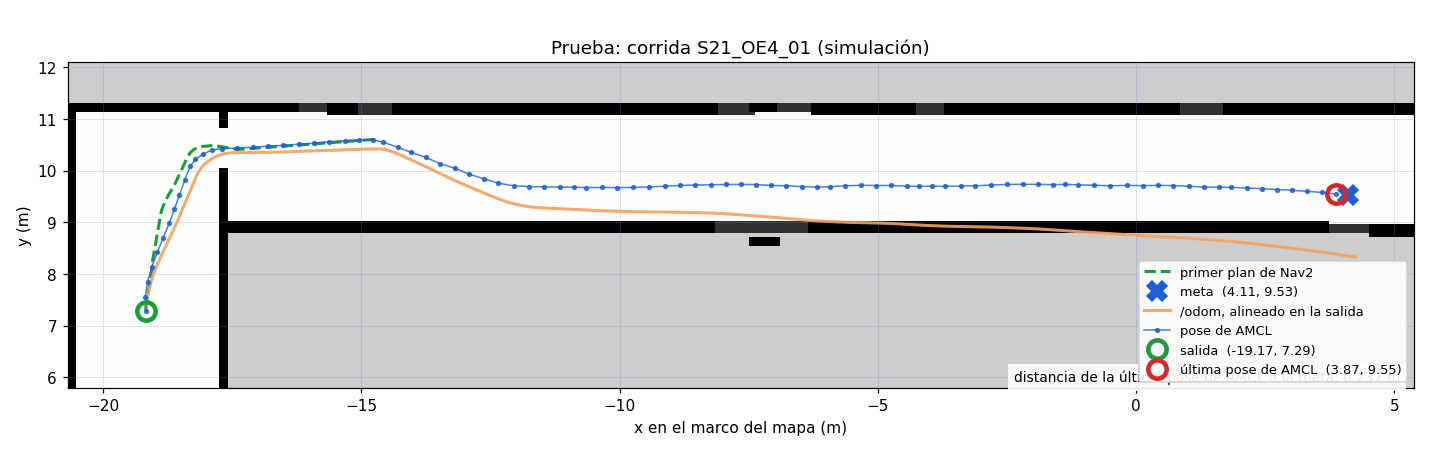
\includegraphics[width=\textwidth]{imagenes/corrida_simulacion.png}
  \caption{Una misión de la campaña en simulación. Se superponen el primer plan
    que calcula el navegador, la pose estimada a lo largo del recorrido y la
    odometría cruda. La separación creciente entre las dos últimas es la deriva
    que la localización corrige contra el mapa.}
  \label{fig:simulacion}
\end{figure}

\section{Evaluación sobre hardware}

\begin{notaavance}[G-2 cerrada el 5 de octubre; G-3 sigue abierta]
De las dos compuertas que esta sección tiene que responder, una cerró y la otra
no, así que se reportan de forma distinta:

\begin{itemize}[leftmargin=*,nosep]
  \item \textbf{G-2, la odometría}, quedó \textbf{alcanzada} en el acta de
    directores del 5 de octubre de 2026, con las medidas del 2 de octubre en el
    piso 4. Sus cifras son definitivas y se reportan en el §4.2.1.
  \item \textbf{G-3, la precisión de llegada}, \textbf{no se alcanzó} en el
    corte C-1 y sigue abierta. El §4.2.2 queda sin redactar: la toma de datos
    continúa hasta el corte del \textbf{16 de octubre}, y escribir ahora unas
    cifras que van a cambiar obligaría a corregirlas después.
\end{itemize}
\end{notaavance}

\subsection{La odometría del vehículo (G-2)}

El vehículo no tiene encoders, así que su odometría sale de comparar barridos
sucesivos del láser. Durante meses esa pieza no produjo una medida utilizable.
La tabla~\ref{tab:odometria} reúne lo que se midió en cada entorno:

\begin{table}[H]
  \centering\small
  \caption{Fracción del avance real que registra la odometría, por entorno.}
  \label{tab:odometria}
  \begin{tabular}{@{}lccl@{}}
    \toprule
    \textbf{Entorno} & \textbf{Recorrido} & \textbf{Registrado} & \textbf{Criterio $\pm$10 \%} \\ \midrule
    Pasillo simulado, 46,9 m & largo & 37,9 \% & falla \\
    Pasillos del edificio (piso 1 y 2) & largo & 5,7 \% y 1,3 \% & falla \\
    Hall del piso 2 & 6 m & 73 \% & falla \\
    Cuarto cerrado, empujado a mano & 3 m & 96,3 -- 101,9 \% & \textbf{cumple} \\
    \textbf{Pasillo del piso 4} & \textbf{6,68 m} & \textbf{95,4 \%} & \textbf{cumple} \\
    \textbf{Pasillo del piso 4} & \textbf{14,57 m} & \textbf{103,3 \%} & \textbf{cumple} \\ \bottomrule
  \end{tabular}
\end{table}

La lectura importa más que las cifras. \textbf{El estimador no mejoró: cambió el
entorno.} En un pasillo recto y uniforme la información de avance no está en el
dato del sensor, y ningún ajuste la recupera. En un pasillo con hornacinas,
lockers y quiebres —ocho cambios de perfil en 25~m— la misma odometría, sin tocar
un parámetro, queda dentro del $\pm$5~\%.

Sobre esas dos últimas filas, las del piso 4, los directores declararon
\textbf{G-2 alcanzada}. Es la compuerta que el proyecto llevaba desde septiembre
señalando como su única ruta crítica.

\subsection{La navegación y la precisión de llegada (G-3), pendientes}

\begin{notaavance}[apartado sin redactar: la toma de datos cierra el 16 de
octubre de 2026]
Aquí irán dos cosas, y ninguna se adelanta:

\begin{enumerate}[leftmargin=*,nosep]
  \item \textbf{La navegación}: evidencia, a partir del registro de cada
    corrida, de que el planificador traza y el controlador sigue sobre el
    vehículo real.
  \item \textbf{La precisión de llegada} (G-3): distancia medida con flexómetro
    entre la parada del vehículo y el destino del catálogo, contra la tolerancia
    de 0,5~m que fijó el director.
\end{enumerate}

Hay sesiones de campo realizadas y sus medidas están registradas en el
repositorio, pero \textbf{no se reportan todavía como resultado}: G-3 no se
alcanzó en el corte C-1 y la demostración continúa. Lo que haya el 16 de octubre
es lo que se defiende.

Lo que sí está medido, y no depende de cuántas corridas más se hagan, es el
mecanismo que condiciona esa llegada: la banda muerta de tracción del vehículo,
documentada en el §3.2.6.
\end{notaavance}

\section{Limitaciones de la medición}
\label{sec:limitaciones}

Tres límites afectan a cómo deben leerse los resultados anteriores. Se declaran
aquí porque callarlos sería presentar como medida lo que no lo es.

\subsection{La continuidad entre niveles es un invariante, no un resultado}

La continuidad del servicio es la variable de respuesta principal del objetivo~4,
y su criterio binario se cumplió en las treinta misiones. \textbf{Ese resultado no
es evidencia de nada}, y la razón es estructural.

El criterio exige que dentro de la ventana de la misión el coordinador nunca esté
en estado inactivo y nunca tenga el agente sin asignar. Los dos únicos puntos del
código que producen esos valores ocurren \emph{antes} de que la ventana se abra.
No existe ejecución posible que lo incumpla: son cero incumplimientos de cero
posibles.

Un criterio que no puede dar resultado negativo no aporta evidencia, por muchas
veces que se verifique. La corrección no fue inventar una ruta de fallo. Eso habría sido instrumentar el
experimento para que pareciera más informativo. Lo que se hizo fue
\textbf{declarar la continuidad como invariante estructural del diseño} y apoyar
la afirmación en una magnitud que sí varía: el hueco temporal del relevo. En las
quince misiones entre niveles tuvo mediana de 0,1~s y máximo de 0,2~s.

\subsection{El intervalo de confianza es ancho por diseño}

Ya se dijo en la tabla~\ref{tab:exito} y se repite porque es el límite más fácil
de olvidar al redactar: con treinta misiones, \textbf{lo defendible es una cota
inferior}, no un valor puntual. Aumentar la confianza exige más muestra, no más
trabajo.

\subsection{El mapa de la campaña leía como libre lo desconocido}

El mapa con que corrió la campaña declaraba un umbral que hacía que
\textbf{10\,908 celdas desconocidas —el 14,5~\% del mapa— se cargaran como
espacio libre}. Con ello, las dos salvaguardas que debían impedir planificar
sobre lo no explorado quedaban desactivadas de hecho.

El alcance de la afirmación, y no más: esto \textbf{no invalida el veredicto}. Los
cuatro fallos fueron de precisión de llegada, no de trazado, y el pasillo por el
que se navegó está mapeado como libre de verdad. Lo que no se sabe es si alguna
trayectoria cruzó una de esas celdas, y es comprobable sobre los registros
conservados. El defecto está corregido desde el 25 de septiembre.
